\subsection{Search tree}
\label{trees}
%add blank space (alinéa)
In order to find the best possible move starting from a position, algorithms build search trees. 
For example, consider Tic-Tac-Toe: \cite{images_annexes}
\begin{figure}[H]
	\centering
	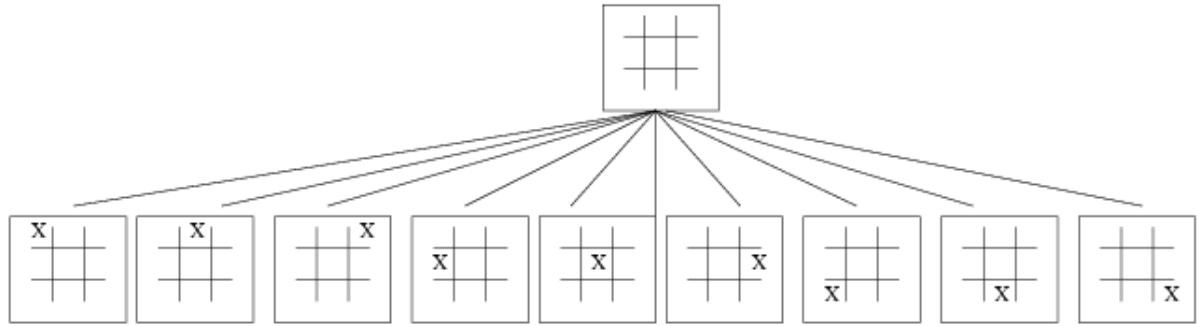
\includegraphics[width=15cm]{3Algorithms/3.1Trees_Benoit/img/Tree1.png}
	\caption{\label{fig:tree1}All possible moves starting from an empty board.}
\end{figure}
\noindent
\begin{figure}[H]
	\centering
	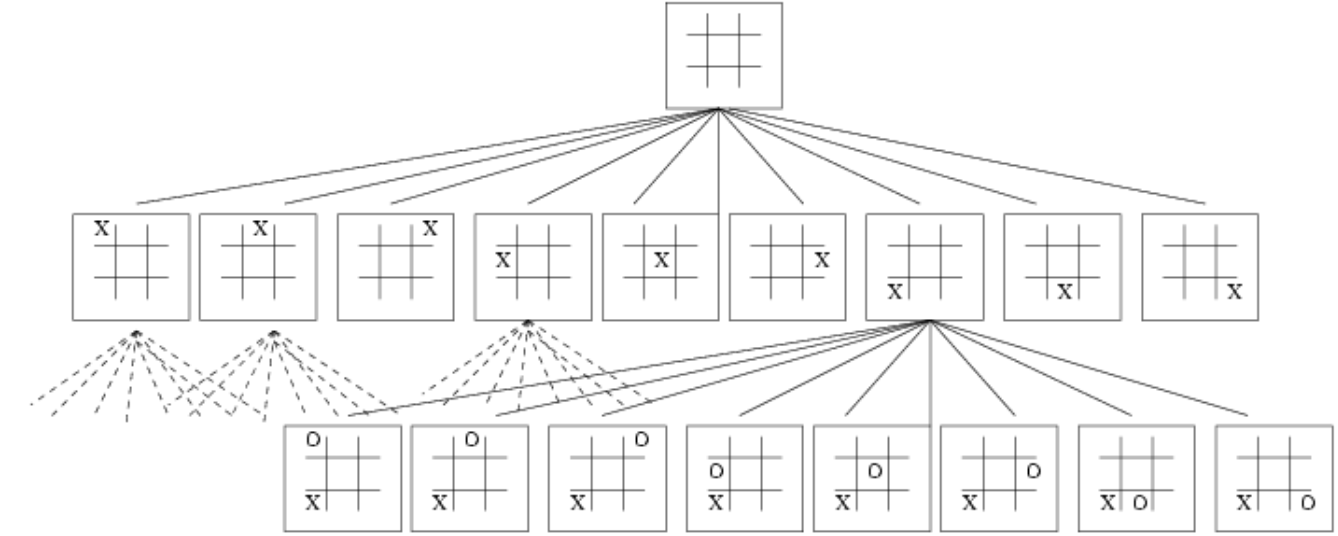
\includegraphics[width=15cm]{3Algorithms/3.1Trees_Benoit/img/Tree2.png}
	\caption{\label{fig:tree2}List of all possible moves for the other player.}
\end{figure}

This expansion is continued until a winning position for the required player is found. Such a tree is called a search tree.
\bigskip\\
However depending on the number of moves possible for the chosen game, the tree might be too large to be explored completely. Therefore in order to simplify the search, the algorithm will try to evaluate the odds of winning in each position that is explored. Those values will be stored in each node and used by the program to find a good move to play from the present position.